\documentclass[11pt]{report}

% Paquetes y configuraciones adicionales
\usepackage{graphicx}
\usepackage[export]{adjustbox}
\usepackage{caption}
\usepackage{float}
\usepackage{titlesec}
\usepackage{geometry}
\usepackage[hidelinks]{hyperref}
\usepackage{titling}
\usepackage{titlesec}
\usepackage{parskip}
\usepackage{wasysym}
\usepackage{tikzsymbols}
\usepackage{fancyvrb}
\usepackage{xurl}
\usepackage{hyperref}
\usepackage{subcaption}

\usepackage{listings}
\usepackage{xcolor}

\usepackage[spanish]{babel}

\newcommand{\subtitle}[1]{
  \posttitle{
    \par\end{center}
    \begin{center}\large#1\end{center}
    \vskip0.5em}
}

% Configura los márgenes
\geometry{
  left=2cm,   % Ajusta este valor al margen izquierdo deseado
  right=2cm,  % Ajusta este valor al margen derecho deseado
  top=3cm,
  bottom=3cm,
}

% Configuración de los títulos de las secciones
\titlespacing{\section}{0pt}{\parskip}{\parskip}
\titlespacing{\subsection}{0pt}{\parskip}{\parskip}
\titlespacing{\subsubsection}{0pt}{\parskip}{\parskip}

% Redefinir el formato de los capítulos y añadir un punto después del número
\makeatletter
\renewcommand{\@makechapterhead}[1]{%
  \vspace*{0\p@} % Ajusta este valor para el espaciado deseado antes del título del capítulo
  {\parindent \z@ \raggedright \normalfont
    \ifnum \c@secnumdepth >\m@ne
        \huge\bfseries \thechapter.\ % Añade un punto después del número
    \fi
    \interlinepenalty\@M
    #1\par\nobreak
    \vspace{10pt} % Ajusta este valor para el espacio deseado después del título del capítulo
  }}
\makeatother

% Configura para que cada \chapter no comience en una pagina nueva
\makeatletter
\renewcommand\chapter{\@startsection{chapter}{0}{\z@}%
    {-3.5ex \@plus -1ex \@minus -.2ex}%
    {2.3ex \@plus.2ex}%
    {\normalfont\Large\bfseries}}
\makeatother

% Configurar los colores para el código
\definecolor{codegreen}{rgb}{0,0.6,0}
\definecolor{codegray}{rgb}{0.5,0.5,0.5}
\definecolor{codepurple}{rgb}{0.58,0,0.82}
\definecolor{backcolour}{rgb}{0.95,0.95,0.92}

% Configurar el estilo para el código
\lstdefinestyle{mystyle}{
  backgroundcolor=\color{backcolour},   
  commentstyle=\color{codegreen},
  keywordstyle=\color{magenta},
  numberstyle=\tiny\color{codegray},
  stringstyle=\color{codepurple},
  basicstyle=\ttfamily\footnotesize,
  breakatwhitespace=false,         
  breaklines=true,                 
  captionpos=b,                    
  keepspaces=true,                 
  numbers=left,                    
  numbersep=5pt,                  
  showspaces=false,                
  showstringspaces=false,
  showtabs=false,                  
  tabsize=2
}

\begin{document}

% Portada del informe
\title{CPU Monociclo}
\subtitle{Diseño de Procesadores}
\author{Carlos Pérez Fino \texttt{alu0101340333@ull.edu.es} \and Cheuk Kelly Ng Pante \texttt{alu0101364544@ull.edu.es}}
\date{\today}
\maketitle

\pagestyle{empty} % Desactiva la numeración de página para el índice

% Índice
\tableofcontents

% Nueva página
\cleardoublepage

\pagestyle{plain} % Vuelve a activar la numeración de página
\setcounter{page}{1} % Reinicia el contador de página a 1

% Secciones del informe
% Capitulo 1
\chapter{Introducción}
En el ámbito del diseño y desarrollo de sistemas digitales, las Field-Programmable Gate Arrays (FPGAs) se han convertido en herramientas esenciales gracias a su flexibilidad y capacidad de reconfiguración. Estos dispositivos permiten la implementación de diversos componentes de hardware programables, lo que posibilita la adaptación y optimización de sistemas en tiempo real. Este informe se centra en la ampliación de una Unidad Central de Procesamiento (CPU) en una FPGA utilizando el lenguaje de descripción de hardware Verilog.

% Capitulo 2
\chapter{Decisiones del diseño}
En nuestro diseño de nuestra CPU ampliada, nos hemos centrado en cubrir en base a lo aprendido las necesidades que se nos exigen en la realización del proyecto intentando hacer de la manera más sencilla y lógica posible. En este proyecto nos hemos basado en que mediante las interrupciones solicitamos que un led se encienda una vez se mantiene el botón que hemos configurado.

% Capitulo 3
\chapter{Camino de datos}
\begin{figure}[H]
  \centering
  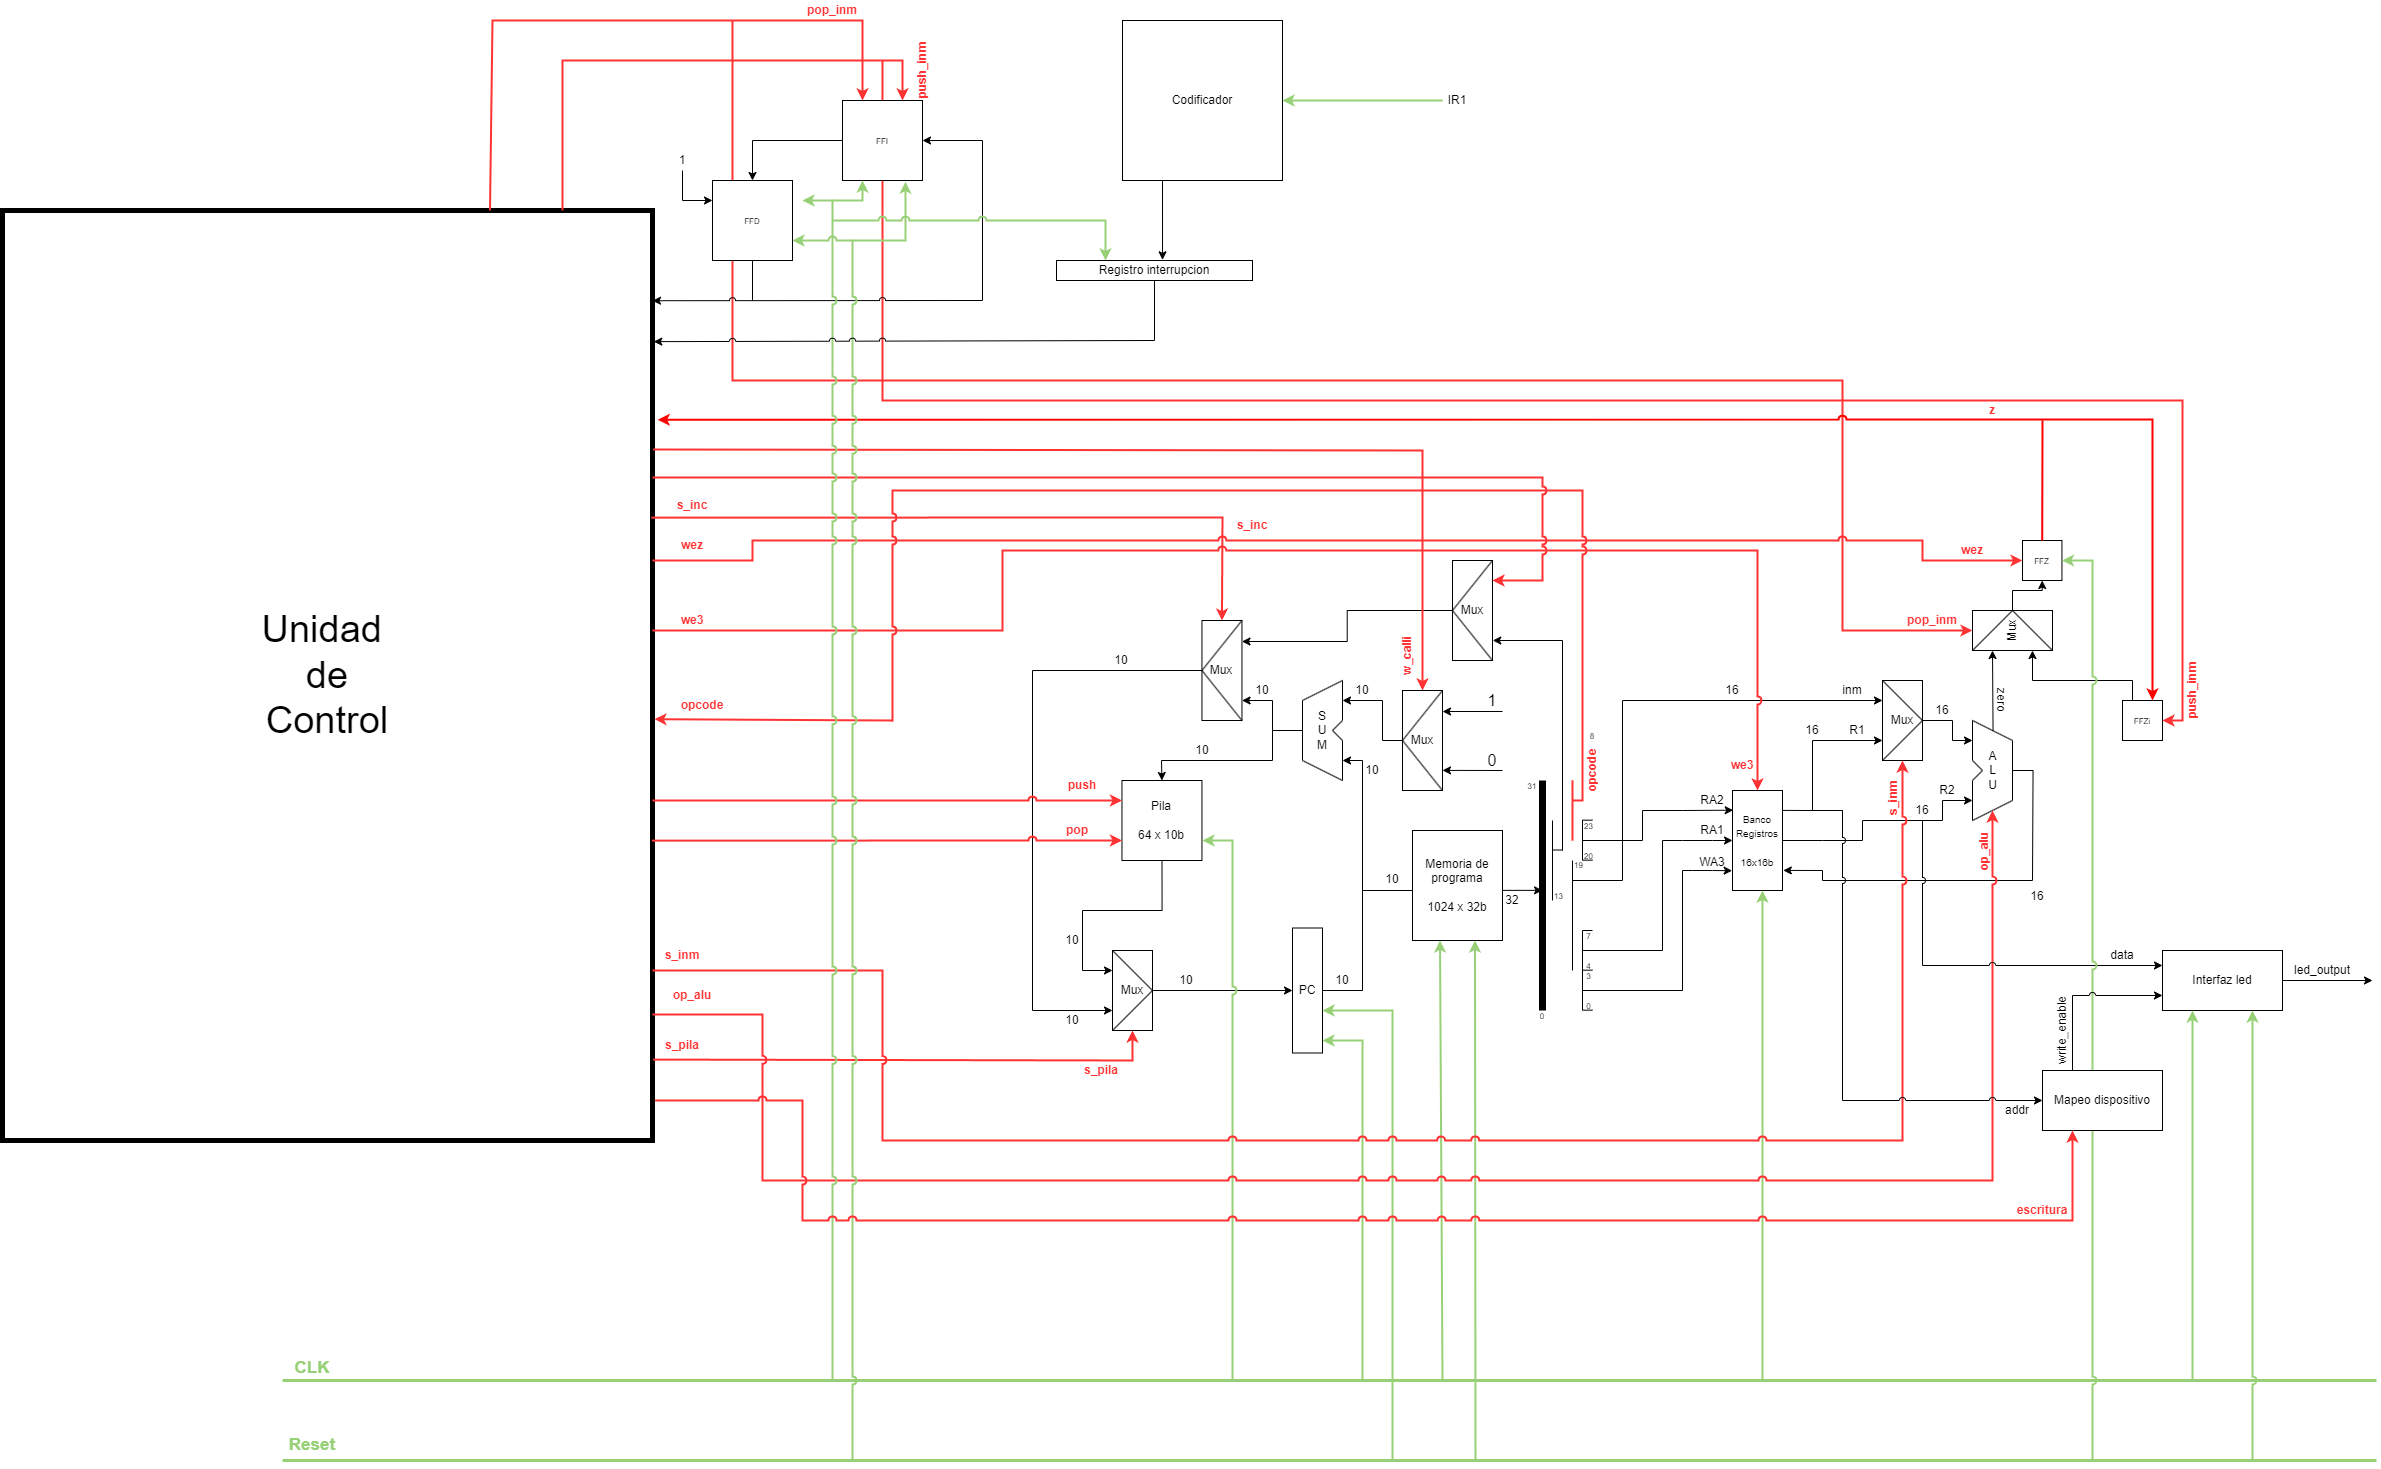
\includegraphics[width=1\textwidth]{img/Camino_datos.png}
  \caption{Camino de datos}
  \label{fig:camino de datos}
\end{figure}

% Capitulo 4
\chapter{Codificación de las instrucciones}
% Tabla de instrucciones 10 x 3
\begin{table}[H]
  \centering
  \begin{tabular}{|c|c|c|}
    \hline
    \textbf{Instrucción}                          & \textbf{OPCODE} & \textbf{Orden en 32  bits} \\ \hline
    \texttt{Aritméticas}                          & 10XXXXXX        & 0-3: Registro destino      \\
                                                  &                 & 4-7: Registro 1            \\
                                                  &                 & 8-19: X                    \\
                                                  &                 & 20-23: Registro 2          \\ \hline
    \texttt{Aritméticas inmediatas}               & 11XXXXXX        & 0-3: Registro destino      \\
                                                  &                 & 4-19: Constante            \\
                                                  &                 & 20-23: Registro 2          \\ \hline
    \texttt{Carga inmediata}                      & 00XXXXXX        & 0-3: Registro destino      \\
                                                  &                 & 4-19: Constante            \\
                                                  &                 & 20-23: Registro 2          \\ \hline
    \texttt{Salto incondicional}                  & 01000100        & 0-3: Registro destino      \\
                                                  &                 & 4-19: Constante            \\
                                                  &                 & 20-23: Registro 2          \\ \hline
    \texttt{Salto si cero}                        & 01001000        & 0-13: X                    \\
                                                  &                 & 14-23: Salto               \\ \hline
    \texttt{Salto si no cero}                     & 01001100        & 0-13: X                    \\
                                                  &                 & 14-23: Salto               \\ \hline
    \texttt{Llamada a subrutina}                  & 01110000        & 0-13: X                    \\
                                                  &                 & 14-23: Salto               \\ \hline
    \texttt{Retorno de subrutina}                 & 01100000        & 0-23: X                    \\ \hline
    \texttt{Retorno de subrutina de interrupcion} & 01111000        & 0-23: X                    \\ \hline
    \texttt{Habilitar escritura entrada/salida}   & 01000000        & 0-3: X                     \\
                                                  &                 & 4-7: Registro 1            \\
                                                  &                 & 8-19: X                    \\
                                                  &                 & 20-23: Registro 2          \\ \hline
  \end{tabular}
  \caption{Codificación de las instrucciones}
  \label{tab:codificación de las instrucciones}
\end{table}

\begin{itemize}
  \item \textbf{Aritmético-lógicas:} La operación de la ALU se encuentra en el \texttt{opcode[5:2]}, donde el registro 1 y el registro 2 son los operadores. Debido a esto hemos añadido a nuestra ALU operaciones adicionales. Que la salida sea igual al segundo operando \texttt{op\_alu = 1001} o poder realizar una resta con el segundo operando menos el primero \texttt{op\_alu = 1000}.
  \item \textbf{Carga inmediata:} Se coge el primer operando que corresponde como constante.
  \item \textbf{Saltos:} Los saltos condicionales se basan en si la última operación de la ALU es 0 o no para realizar el salto.
  \item \textbf{Llamadas a subrutinas:} Saltan a la dirección donde se encuentra la subrutina.
  \item \textbf{Retorno de subrutinas:} Se extrae la dirección de retorno de la pila.
  \item \textbf{Retorno de subrutinas de interrupción:} Se extrae la dirección de retorno de la pila y se vuelven a habilitar las interrupciones.
\end{itemize}

\newpage

% Capitulo 5
\chapter{Características añadidas a diseño final}
\begin{enumerate}
  \item Se ha aumentado el tamaño de los registros a 16 bits.
  \item Se ha aumentado el tamaño de las instrucciones a 32 bits.
  \item Ampliación a instrucciones aritmético-lógicas con datos inmediatos como comentamos anteriormente.
  \item Se ha añadido una pila que almacena direcciones de retorno de subrutinas y de interrupción.
        \begin{itemize}
          \item \textbf{Push:} se escribe la dirección de retorno y se incrementa el stack pointer.
          \item \textbf{Pop:} saca el elemento anterior al stack pointer, lo borra y decrementa el stack pointer.
        \end{itemize}
  \item Se ha añadido un sistema de interrupciones para permitir a los dispositivos externos solicitar atención de la CPU.
        \begin{itemize}
          \item \textbf{Codificador:} Este módulo que hemos creado se encarga de codificar las líneas de interrupción, asignando una prioridad a cada línea de interrupción. Estas líneas se encuentran conectadas a los botones de la FPGA, por lo que se activarán cuando presionemos nuestro botón. En este caso será con el único botón que hemos conectado.
          \item \textbf{Registro\_interrupcion: } Almacena la interrupción hasta que pueda realizarse, esto ocurrirá cuando acabe el flanco de reloj o cuando acabe una interrupción previa.
          \item \textbf{ffi:} Determina si pueden proceder las interrupciones o no.
          \item \textbf{ffd:} Guarda el estado del ffi y lo reenvía al ffi y luego también a la unidad de control.
          \item \textbf{dir\_sal\_in:} Se encarga de darnos una dirección de salto a la que saltar para atender la instrucción requerida, esto sucede cuando nos llega la señal de nuestro botón de la señal ir\_attended.
          \item Hemos añadido señales nuevas para el control de las interrupciones:
                \subitem \textbf{pop\_inm:} Se encarga de indicar cuando se tiene que habilitar de nuevo las interrupciones.
                \subitem \textbf{push\_inm:} Se encarga de indicar cuando una interrupción tiene que ser atendida.
                \subitem \textbf{wcalli:} Se utiliza para saber que dirección de salto se debe seleccionar.
          \item Se han añadido 3 funciones adicionales para el flag de cero de nuestra ALU, esto lo hemos tenido que hacer para poder mantener dicho flag cuando tenemos que retornar de la subrutina.
                \subitem \textbf{ffzi:} Este biestable tipo d guarda el estado del flag de cero.
                \subitem \textbf{zero\_guard:} Este mux se encarga de restaurar el flag cuando tengamos que retornar de la interrupción.
        \end{itemize}
  \item Se ha añadido un sistema de buses exteriores.
        \begin{itemize}
          \item \textbf{addr:} Bus de direcciones de 16 bits. Se ha conectado al registro 1 donde se indica que led se enciende.
          \item \textbf{data:} Bus de datos de 16 bits. Se ha conectado al registro 2 donde se indica el valor a escribir.
          \item \textbf{mapeo\_dis:} Este módulo parte de la dirección del bus de direcciones, donde se obtiene el led que se pretende escribir, esto se hace mediante la señal \textbf{“escritura”} que habilita la escritura en mapeo\_dis.
          \item \textbf{interfaz\_led:} Este módulo tiene una salida hacia un led de la placa, donde se produce un mapeo del valor de bus de datos a un valor que puede ser alto o bajo.
        \end{itemize}
\end{enumerate}

% Capitulo 6
\chapter{Programa}
Hemos realizado un programa donde cargamos un valor se realiza una resta, luego se hace un salto a una subrutina donde se realiza otra resta. Además, también tenemos el código  donde se muestra el uso de las interrupciones para encender el led que tenemos.
\begin{figure}[H]
  \centering
  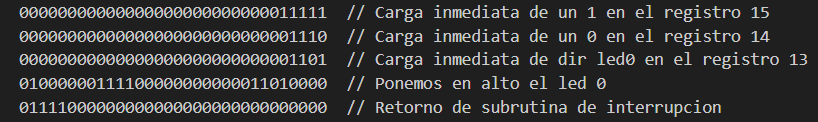
\includegraphics[width=1\textwidth]{img/Programa_Binario.png}
\end{figure}

\begin{figure}[H]
  \centering
  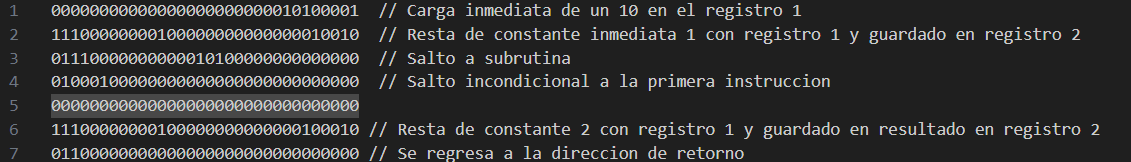
\includegraphics[width=1\textwidth]{img/Programa.png}
\end{figure}


\chapter{Demostración}
\begin{itemize}
  \item Simulación RTL, hemos realizado dos simulaciones para verificar el programa:
  \begin{figure}[H]
    \centering
    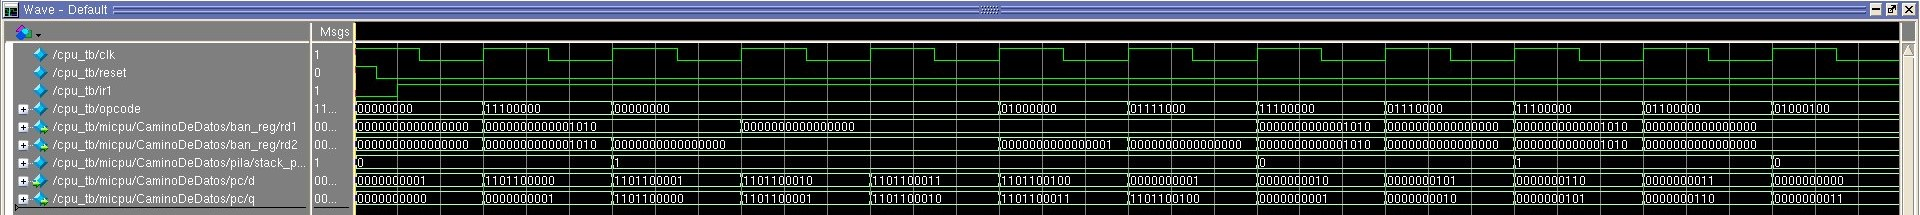
\includegraphics[width=1\textwidth]{img/error_prueba_ejemplos_TCM1.jpeg}
  \end{figure}
  
  \begin{figure}[H]
    \centering
    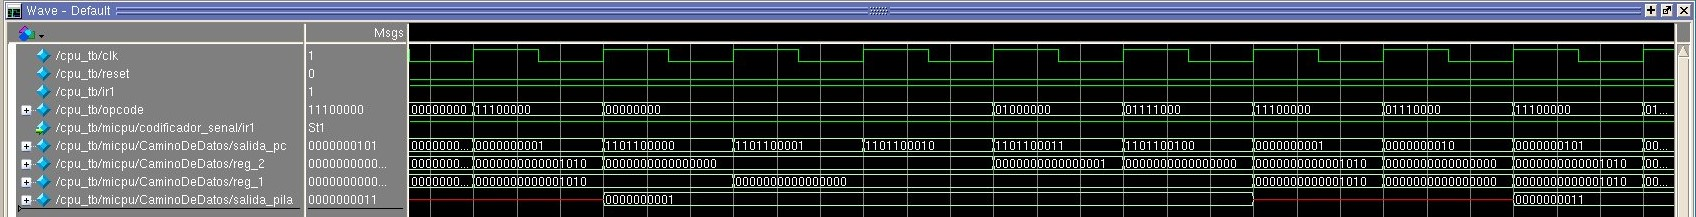
\includegraphics[width=1\textwidth]{img/segundaSimRTL.jpeg}
  \end{figure}
  
  Aquí podemos observar cómo se producen las cargas inmediatas, resta, y el salto a la subrutina que hemos creado. Además, podemos observar el funcionamiento de nuestra pila.

  \item La simulación Slow Model para verificar el comportamiento de nuestro programa, debido a las limitaciones que nos daba el Slow Model, debido a que no nos dejaba manejar más señales, en comparación con el RTL lo comprobaremos en base al opcode:
  \begin{figure}[H]
    \centering
    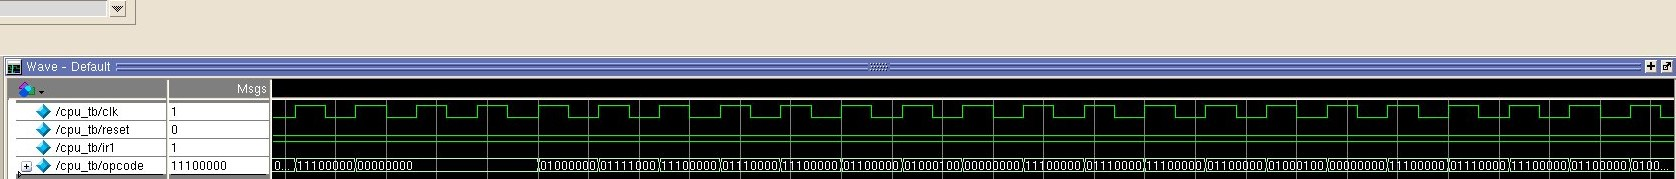
\includegraphics[width=1\textwidth]{img/SlowModel.jpeg}
  \end{figure}

  \item Resultados que hemos obtenido con el Slow Model:
  \begin{figure}[H]
    \centering
    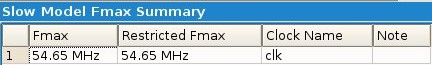
\includegraphics[width=1\textwidth]{img/frecuencia.jpeg}
  \end{figure}

  \begin{figure}[H]
    \centering
    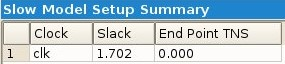
\includegraphics[width=1\textwidth]{img/setupSummary.jpeg}
  \end{figure}


\end{itemize}

\chapter*{Enlace al video}
\url{https://www.youtube.com/shorts/RaqYaGooHBU}

\end{document}